\documentclass[italian,a4paper]{article}
\usepackage[tight,nice]{units}
\usepackage{babel,amsmath,amssymb,amsthm,graphicx,url}
\usepackage[text={5.5in,9in},centering]{geometry}
\usepackage[utf8x]{inputenc}
\usepackage[T1]{fontenc}
\usepackage{ae,aecompl}
\usepackage[footnotesize,bf]{caption}
\usepackage[usenames]{color}
\usepackage{textcomp}
\usepackage{gensymb}
%\include{pstricks}
\frenchspacing
\pagestyle{plain}
%------------- eliminare prime e ultime linee isolate
\clubpenalty=9999%
\widowpenalty=9999
%--- definizione numerazioni
\renewcommand{\theequation}{\thesection.\arabic{equation}}
\renewcommand{\thefigure}{\arabic{figure}}
\renewcommand{\thetable}{\arabic{table}}
\addto\captionsitalian{%
  \renewcommand{\figurename}%
{Grafico}%
}
%
%------------- ridefinizione simbolo per elenchi puntati: en dash
%\renewcommand{\labelitemi}{\textbf{--}}
\renewcommand{\labelenumi}{\textbf{\arabic{enumi}.}}
\setlength{\abovecaptionskip}{\baselineskip}   % 0.5cm as an example
\setlength{\floatsep}{2\baselineskip}
\setlength{\belowcaptionskip}{\baselineskip}   % 0.5cm as an example
%--------- comandi insiemi numeri complessi, naturali, reali e altre abbreviazioni
\renewcommand{\leq}{\leqslant}
%--------- porzione dedicata ai float in una pagina:
\renewcommand{\textfraction}{0.05}
\renewcommand{\topfraction}{0.95}
\renewcommand{\bottomfraction}{0.95}
\renewcommand{\floatpagefraction}{0.35}
\setcounter{totalnumber}{5}
%---------
%
%---------
\begin{document}
\title{Relazione di laboratorio: reticolo di diffrazione}
\author{\normalsize Ilaria Brivio (582116)\\%
\normalsize \url{brivio.ilaria@tiscali.it}%
\and %
\normalsize Matteo Abis (584206)\\ %
\normalsize \url{webmaster@latinblog.org}}
\date{\today}
\maketitle
%------------------
\section{Obiettivo dell'esperienza}
L'obiettivo dell'esperienza è la stima delle lunghezze d'onda della luce emessa da una lampada al cadmio, mediante lo studio della figura di diffrazione prodotta da un reticolo a molte fenditure.

\section{Descrizione dell'apparato strumentale}
L'apparato è costituito da un reticolo di diffrazione di passo
$a=\unit[12.65 \pm 0.05]{\micro m}$ che può ruotare attorno a un asse fisso.
Allo stesso asse è vincolato un cannocchiale attraverso il quale vengono
osservati i raggi luminosi. Al sostegno di ciascun elemento è inoltre
fissato uno dei due dischi concentrici di un nonio di sensibilità 2', che
permette di misurare l'angolo tra le posizioni del reticolo e del
cannocchiale. Per eliminare l'errore di eccentricità sono presenti due
nonii, $A$ e $B$, diametralmente opposti, cosicc\'e le loro misure differiscono di 180\textdegree.

Le posizioni del reticolo e del cannocchiale possono essere regolate con precisione grazie ad apposite chiavi micrometriche e l'immagine può essere ottimizzata agendo su un diaframma posto davanti alla sorgente e sulle lenti del cannocchiale.

Sul reticolo incide la luce prodotta da una lampada al cadmio, che emette radiazioni di colore rosso, verde, blu chiaro (che chiameremo blu 2), blu scuro (blu 1) e violetto. In quest'esperienza è stata però trascurata la componente nel violetto, che risultava troppo poco visibile.

\section{Descrizione della metodologia di misura}
\subsection*{Ortogonalizzazione del reticolo}
Prima di realizzare le misure ci si è assicurati che il fascio luminoso incidesse ortogonalmente al reticolo di diffrazione. Una seppur piccola asimmetria può infatti essere fonte di un errore sistematico sulla determinazione della lunghezza d'onda.

Si è dapprima stabilita una posizione di "azzeramento" dei nonii, calcolando una media dei due valori indicati quando il cannocchiale è allineato con il fascio incidente. Si è poi spostato il cannocchiale di 90\textdegree~in senso antiorario ed è stato ruotato il reticolo, lasciando però fissi i nonii, fino a vedere il raggio riflesso nel cannocchiale.

L'operazione è stata ripetuta portando il cannocchiale dall'altro lato, sempre a 90\textdegree~dall'asse di zero, e facendo ruotare il reticolo assieme ai nonii: il raggio riflesso è visibile quando l'angolo rispetto alla posizione precedente è di 90\textdegree 6' secondo il nonio $A$ e di 269\textdegree 54' secondo il nonio $B$.

Dopo aver ruotato nuovamente il cannocchiale di 90\textdegree in senso orario, si è portato infine lo schermo indietro di 45\textdegree 3', pari alla metà dell'angolo tra le due posizioni precedenti.

Nella posizione di allineamento del cannocchiale con il massimo centrale di interferenza i nonii riportano i valori $\theta_A=$ 45\textdegree 14' e $\theta_B=$ 225\textdegree 6'.
\subsection*{Misure sui raggi diffratti}
Tenendo fisso il reticolo, si è spostato gradualmente il cannocchiale allontanandolo dalla posizione di zero, e sono stati registrati i valori riportati dai nonii quando una linea colorata, corrispondente a un massimo di interferenza, era visibile al centro dell'oculare.
In questo modo sono stati misurati gli angoli di deflessione dei massimi fino al quinto ordine per le tre lunghezze d'onda minori, e solo fino al quarto per il rosso, dato che il massimo del quinto ordine risultava troppo poco visibile.
\subsection*{Errori sistematici}
Le principali fonti di errore sistematico nell'esperienza sono l'eccentricità dell'asse di rotazione dei nonii e la mancata ortogonalizzazione del reticolo.

La prima è dovuta al fatto che le misure degli angoli fornite dai nonii sono indirette: la grandezza misurata direttamente è infatti la lunghezza dell'arco di circonferenza sotteso dall'angolo stesso e di conseguenza il fattore di conversione dipende strettamente dalla distanza della scala graduata dall'asse di rotazione. Se l'asse non passa esattamente per il centro della circonferenza si commette allora un errore sistematico tanto maggiore quanto più ampia  la rotazione. Con un semplice studio geometrico si può verificare che tale errore è completamente eliminato se si usano due nonii in posizioni diametralmente opposte e si assume come misura dell'angolo la media dei due valori indicati.

La mancata ortogonalizzazione del reticolo rispetto alla direzione del fascio incidente, invece, è causa di una differenza di fase aggiuntiva tra i raggi che partono da due fenditure adiacenti. Ciò si traduce in un'asimmetria tra gli angoli di deflessione alla destra e alla sinistra dell'asse centrale e la stima di $\lambda$ risulta infine alterata di un certo fattore moltiplicativo.

\section{Risultati sperimentali ed elaborazione dati}
Per ciascun massimo è stato calcolato l'angolo di deviazione $\theta$ come valor medio tra le misure dei due nonii. Tale valore è stato poi convertito da gradi in radianti.
\begin{equation*}
\theta=\dfrac{(\theta_A-180)+\theta_B}{2}\cdot\dfrac{\pi}{180}
\end{equation*}
Come noto dallo studio teorico di questi fenomeni di interferenza, la posizione $\theta_n$ del massimo di ordine $n$ è legata alla lunghezza d'onda $\lambda$ e al passo del reticolo $a$ dalla relazione:
\begin{equation*}
\sin\theta_n=n\dfrac{\lambda}{a}
\end{equation*}
Per ogni lunghezza d'onda è stato allora realizzato un grafico con numero d'ordine in ascissa e $\sin\theta$ in ordinata ed è stato eseguito un fit lineare con una retta $y=mx+c$. (Grafici \ref{1blu}, \ref{2blu}, \ref{verde}, \ref{rosso}).
Dal coefficiente angolare si è infine stimata la lunghezza d'onda $\lambda=a m$, con errore ottenuto sommando in quadratura.

\newpage
I risultati ottenuti sono riportati nella tabella seguente. Riportiamo anche
un confronto con i valori attesi:
\begin{table}[!h]
\centering
\renewcommand{\arraystretch}{1.3}
\begin{tabular}{cr@{ $\pm$ }l c}
colore&	\multicolumn{2}{c}{$\lambda (\unit{nm})$} &
$\lambda_{\text{veri}} (\unit{nm})$\\\hline
blu 1& 		474.3& 2.2 &467.8\\
blu 2& 		489.6& 1.9 &480.0\\
verde& 		517.2& 2.1 &508.6\\
rosso& 		656.7& 2.7 &643.8\\
\end{tabular}
\end{table}

Si osserva la presenza di un errore sistematico di circa \unit[10]{nm} in eccesso su tutti i risultati ottenuti.

Possiamo escludere che tale errore sia dovuto a un'errata ortogonalizzazione
del reticolo, dato che le figure di diffrazione non presentano asimmetrie.
Inoltre l'errore si è presentato con le stesse modalità anche ripetendo le
misure una seconda volta, procedendo daccapo
all'ortogonalizzazione, e considerando i massimi della luce blu 1 fino al sesto ordine (Grafico \ref{1nblu}).

Non si è osservata alcuna differenza nemmeno nel prendere le misure spostando il cannocchiale dal centro verso l'esterno per entrambi i lati piuttosto che partendo da uno dei due massimi più lontani per poi muovere il cannocchiale sempre nello stesso senso. Ciò sembra quindi escludere anche questioni di tolleranze meccaniche nell'apparato.

Abbiamo dunque pensato che l'errore fosse dovuto a un'errata determinazione
del passo del reticolo. Dagli stessi grafici abbiamo dunque ricavato la
distanza tra le fenditure, utilizzando le lunghezze d'onda note dello
spettro. 
\begin{table}[!h]
\centering
\renewcommand{\arraystretch}{1.3}
\begin{tabular}{cr@{ $\pm$ }l}
colore&	\multicolumn{2}{c}{$a (\unit{\micro m})$} \\\hline
blu 1& 		17.61& 0.08 \\
blu 2& 		17.59& 0.07 \\
verde& 		17.62& 0.07 \\
rosso& 		17.58& 0.07 \\
\end{tabular}
\end{table}\\
La consistenza tra queste determinazioni è certamente convincente. Si può
quindi stimare la separazione tra le fenditure di questo reticolo con una
media pesata come $a=\unit[17.60\pm0.04]{\micro m}$.
\newpage
\section{Appendice}
\subsection*{Grafici}
\begin{figure}[!h]\centering
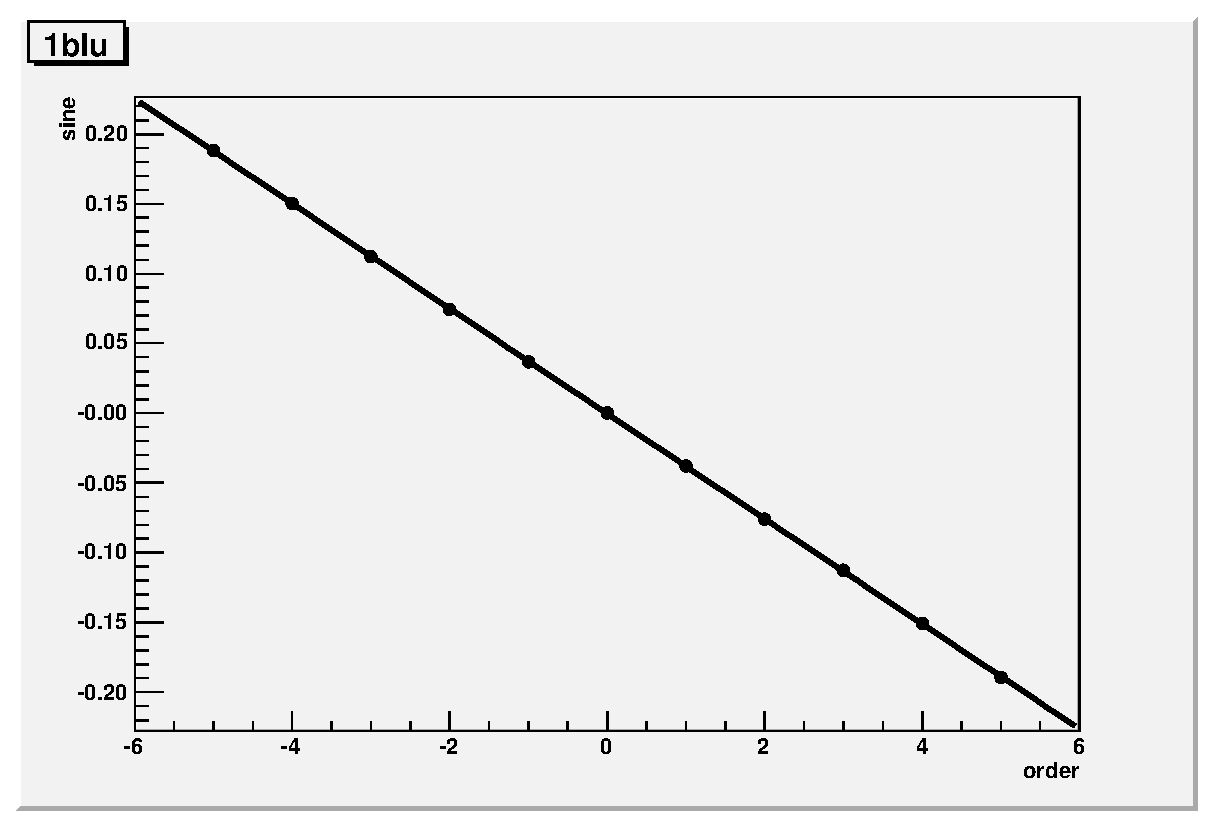
\includegraphics[width=\textwidth]{1blu.eps}
\caption{Luce blu scuro. Grafico con numero d'ordine del massimo di interferenza in ascissa e seno dell'angolo di deflessione in ordinata. Di seguito sono riportati i residui dell'interpolazione.}\label{1blu}
\end{figure}
\begin{figure}[!h]\centering
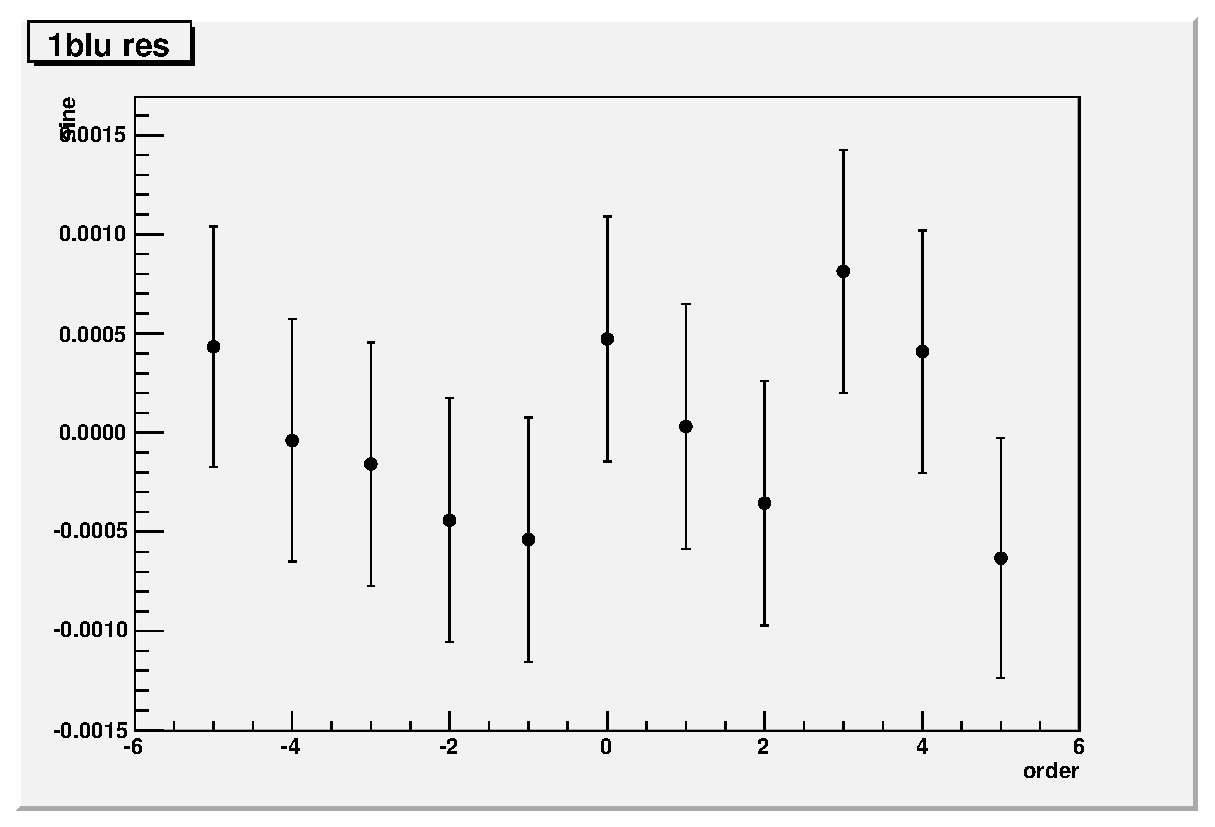
\includegraphics[width=\textwidth]{1blu.res.eps}
\end{figure}
\begin{figure}[!h]\centering
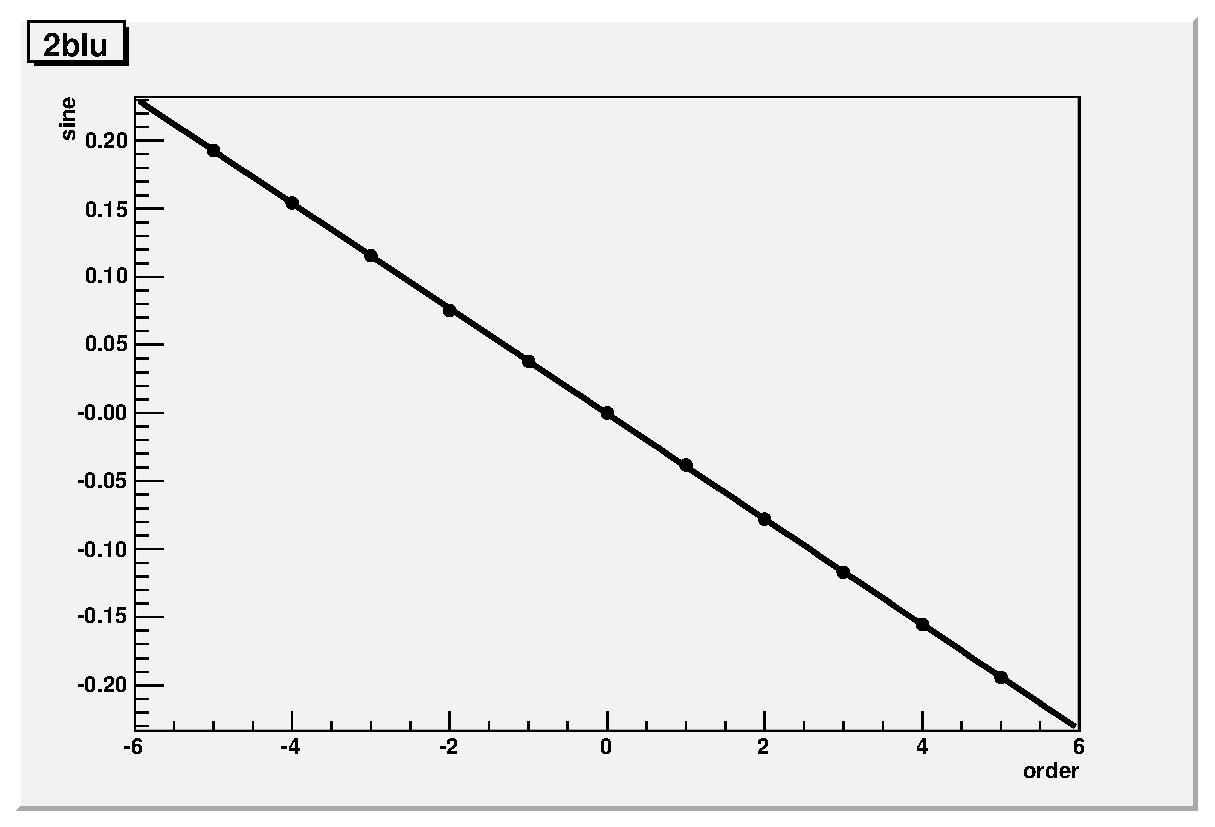
\includegraphics[width=\textwidth]{2blu.eps}
\caption{Luce blu chiaro. Grafico con numero d'ordine del massimo di interferenza in ascissa e seno dell'angolo di deflessione in ordinata. Di seguito sono riportati i residui dell'interpolazione.}\label{2blu}
\end{figure}
\begin{figure}[!h]\centering
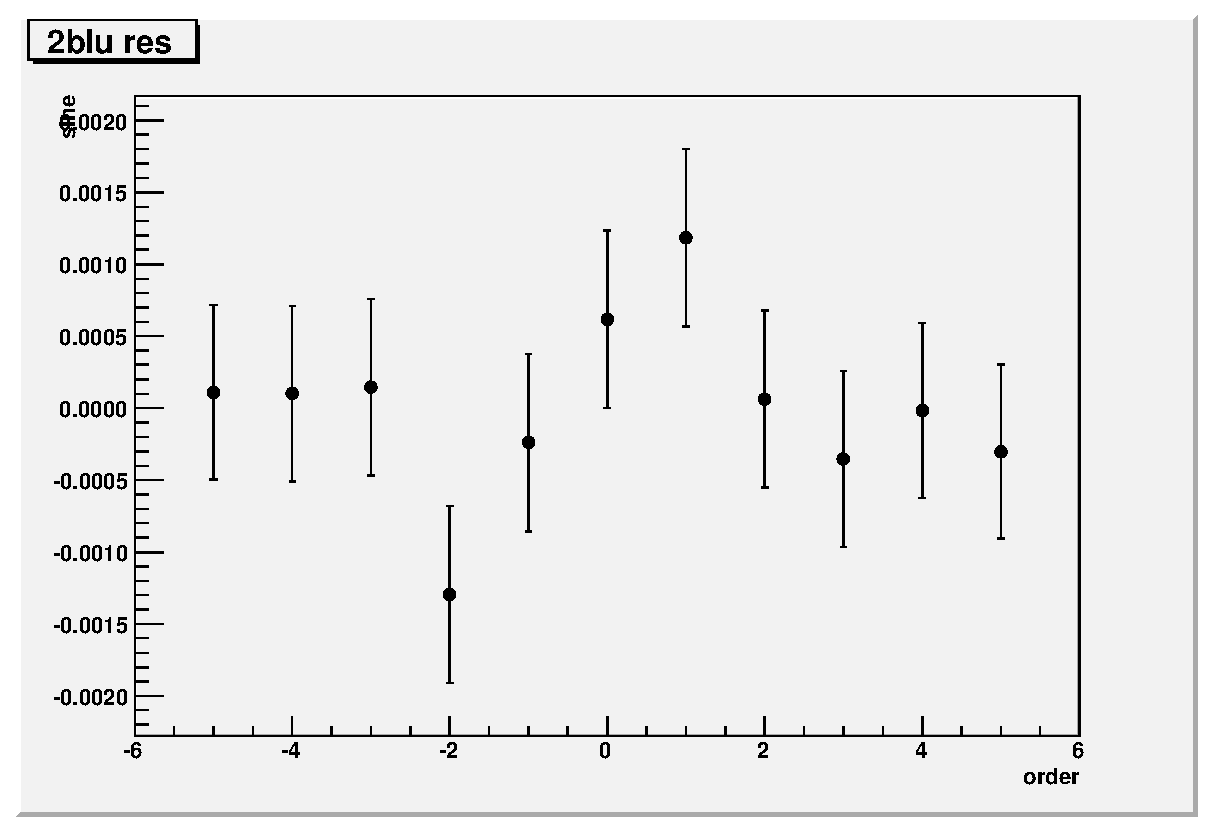
\includegraphics[width=\textwidth]{2blu.res.eps}
\end{figure}
\begin{figure}[!h]\centering
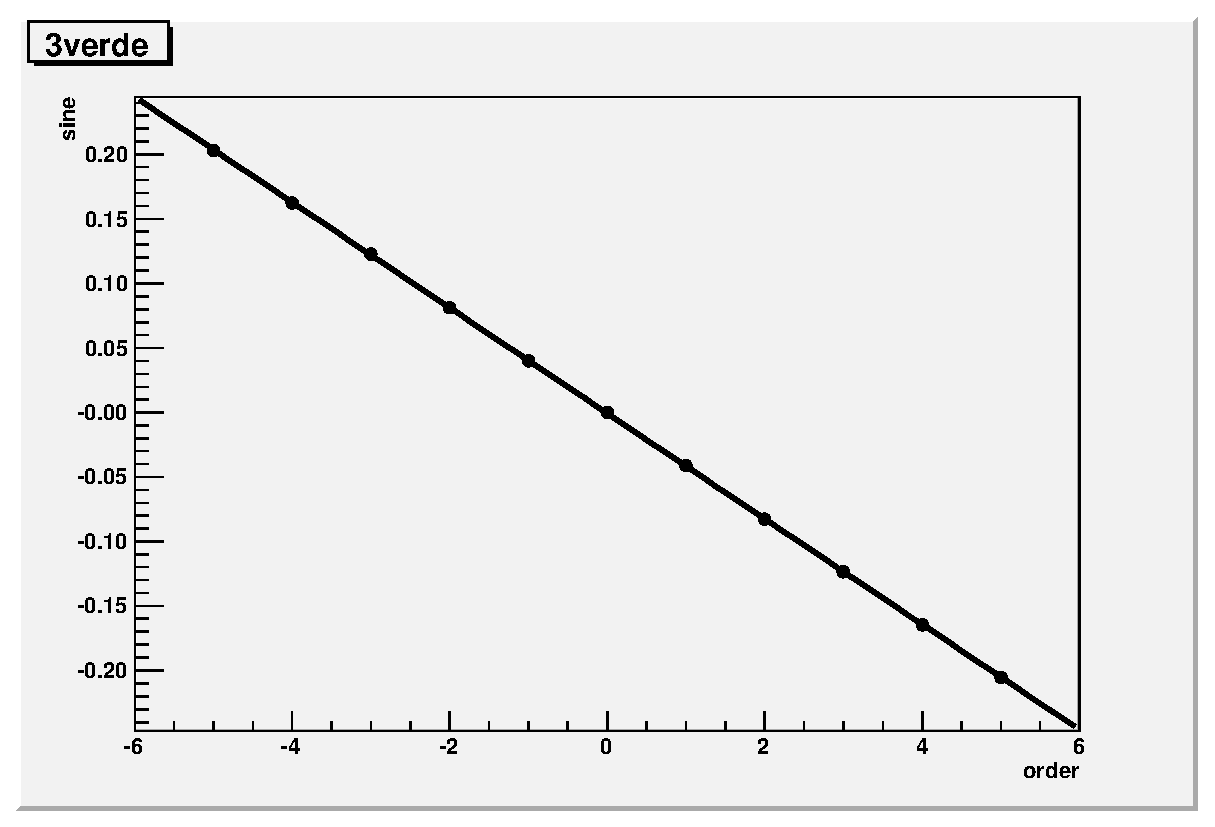
\includegraphics[width=\textwidth]{3verde.eps}
\caption{Luce verde. Grafico con numero d'ordine del massimo di interferenza in ascissa e seno dell'angolo di deflessione in ordinata. Di seguito sono riportati i residui dell'interpolazione.}\label{verde}
\end{figure}
\begin{figure}[!h]\centering
\includegraphics[width=\textwidth]{3verde.res.eps}
\end{figure}
\begin{figure}[!h]\centering
\includegraphics[width=\textwidth]{4rosso.eps}
\caption{Luce rossa. Grafico con numero d'ordine del massimo di interferenza in ascissa e seno dell'angolo di deflessione in ordinata. A differenza dei grafici precedenti, qui ci si è fermati al quarto ordine poiché il quinto risultava poco visibile. Di seguito sono riportati i residui dell'interpolazione.}\label{rosso}
\end{figure}
\begin{figure}[!h]\centering
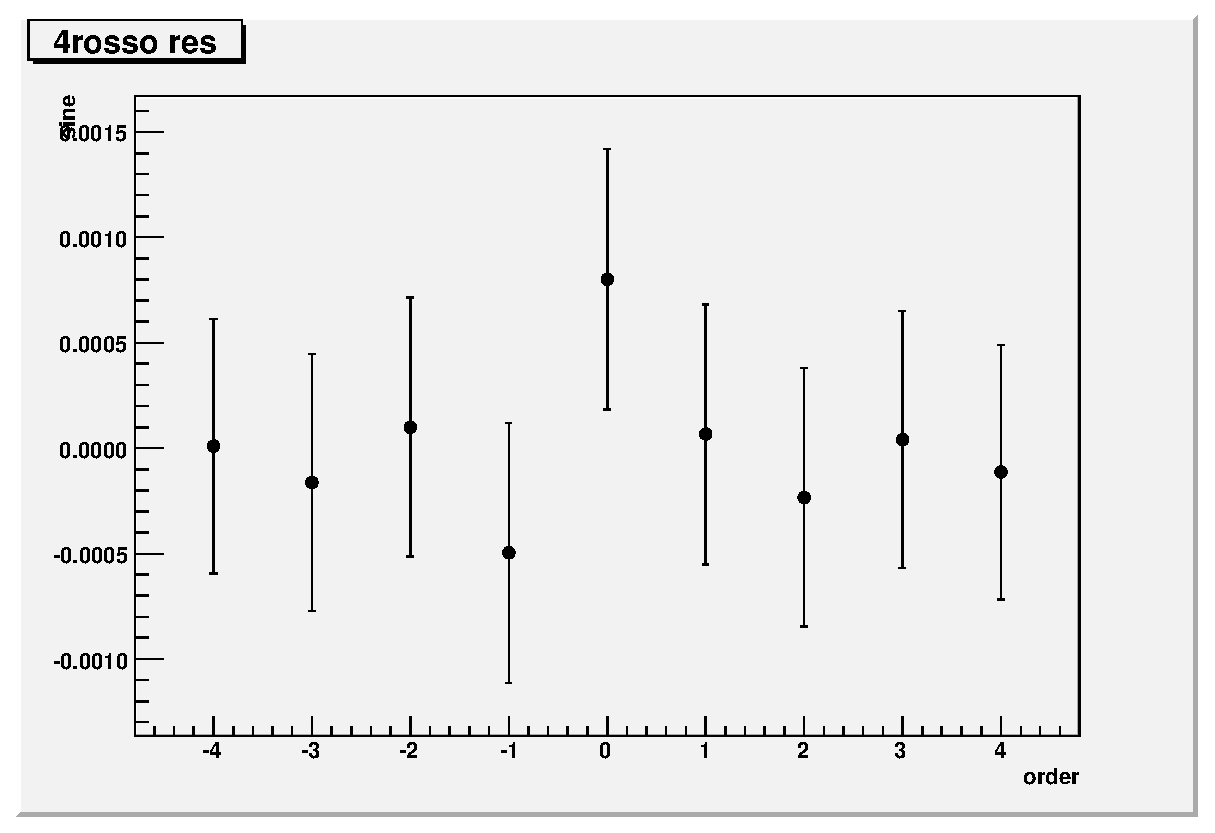
\includegraphics[width=\textwidth]{4rosso.res.eps}
\end{figure}
\begin{figure}[!h]\centering
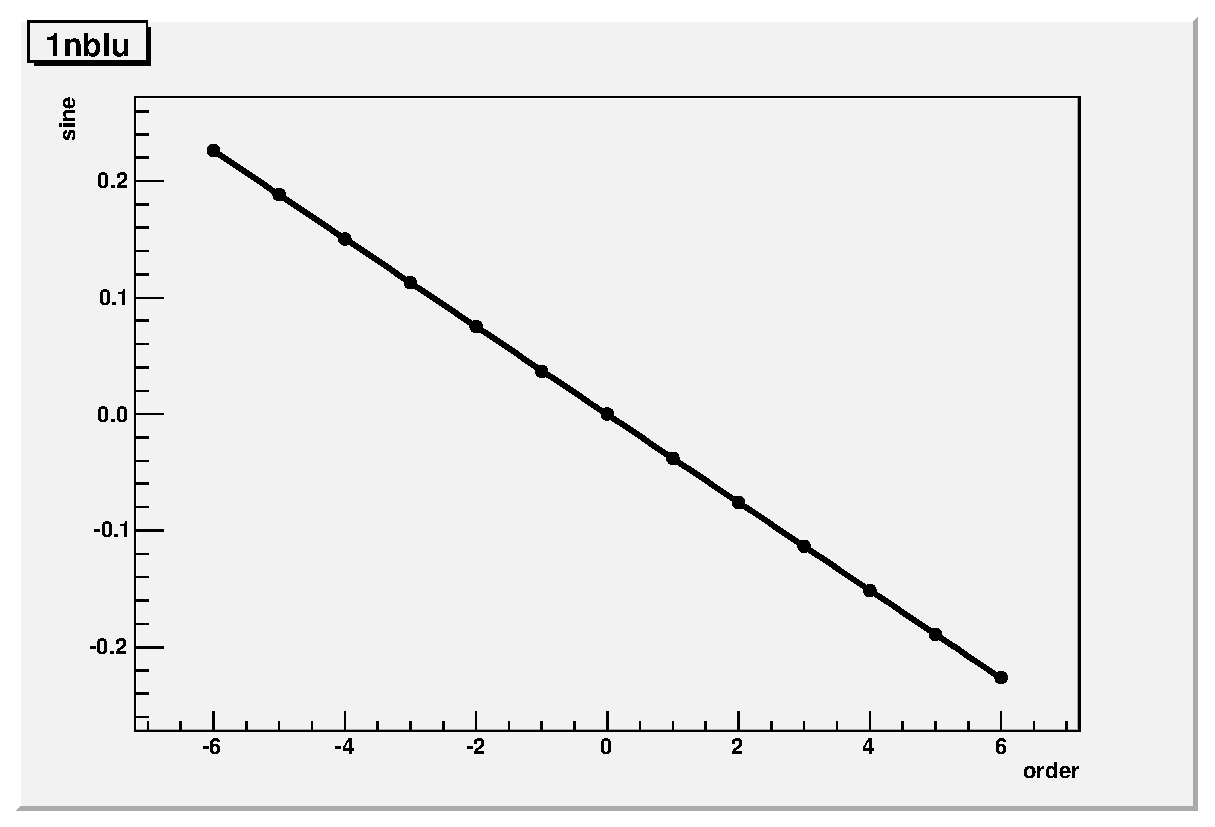
\includegraphics[width=\textwidth]{1nblu.eps}
\caption{Grafico realizzato per la seconda serie di misure con la luce blu scuro e fino al massimo del sesto ordine. Come sopra, in ascissa c'è il numero d'ordine del massimo di interferenza e in ordinata il seno dell'angolo di deflessione. Di seguito sono riportati i residui dell'interpolazione.}\label{1nblu}
\end{figure}
\begin{figure}[!h]\centering
\includegraphics[width=\textwidth]{1nblu.res.eps}
\end{figure}
\end{document}
